\section{Graded Assignment 3}\label{sec:graded_assignment_3}

% A full answer and result analysis is expected for task 3 and 4. For task 3 you should include a plot of the pose over time as well as the final estimated landmarks for your choice of parameters, in addition to NEES and NIS over time for the same set of parameters. In task 4 the same plots are expected, where the GPS can be used for ground truth. For both tasks it should be made clear why the parameters were chosen in terms of error metrics, consistency and overall result. Answers and analysis should connect theory and results to the real world, and show your understanding for the problem and solution. Try to connect the results on the simulated data to the results of the read data where and if it is possible. 

An extended Kalman filter was implemented for solving the SLAM problem in MATLAB. Specifically, the EKF-SLAM formulation in this report considers only the 2D case, with odometer measurements acting as control input. Furthermore, data association is done with the JCBB algorithm. For the relevant theory behind this EKF-SLAM formulation and JCBB, consult \cite[p. 185 - 196]{Edmund}.

\subsection{EKF-SLAM on simulated vehicle data set}

% Q, R, JCBB alphas
% NIS. Pose and lmks close to GT.

%The overall target was to minimize the difference between the estimated position and the ground truth, as well as decent NIS over time. Specifically we calculated the confidence interval over time with the size of the current innovation as the number of degrees of freedom. Initially, we set the noise covariance matrices higher than necessary, to get a rather conservative result, and decreased them as appropriatly. At the same time, we decreased the alphas used in the JCBB, as we could assume most of the measurements were from real landmarks. This resulted in a decently quick script, with the estimates being very close to the ground truth (with few / small offsets) and a decent NIS over time. 

The EKF-SLAM was first tuned using a simulated vehicle data set. The odometer measurement noise was tuned according to $Q = \text{diag}(\begin{array}{ccc}[(\sigma_u^2 & \sigma_v^2 & \sigma_\varphi^2 ]^{\top})\end{array}$, where $\sigma_u = \sigma_v = \SI{1e-1}{\meter\per\second}$ and $\sigma_\varphi = \SI{1e-2}{rad}$. The range-bearing measurement noise covariance was tuned according to $R = \text{diag}(\begin{array}{cc}[\sigma_r^2 & \sigma_\theta^2 ]^{\top})\end{array}$, where $\sigma_r = \SI{4e-2}{\meter}$ and $\sigma_\theta = \SI{2e-2}{rad}$. The JCBB algorithm was tuned by letting the individual compatability significance level be $\alpha_{ic} = \SI{1e-5}{}$ and the joint compatabiltiy significance level be $\alpha_{jc} = \SI{1e-10}{}$.

The system was tuned by trying to minimize the errors in pose and landmark estimates, while also looking at the calculated total NIS and NEES in pose. Note that in the NIS case the confidence interval was calculated at each time step, using the size of the current innovation as the number of degrees of freedom in the $\chi^2$ distribution. The estimated pose trajectory and landmark positions are presented in \cref{fig:ga_3_sim_trajectory}, and the consistency analysis plots are presented in \cref{fig:ga_3_sim_NIS}. We observe that 90\% of the NIS is inside the calculated the confidence interval, while 94.6\% of the NEES is inside the confidence intervals.

\begin{figure}[!htb]
    \centering
    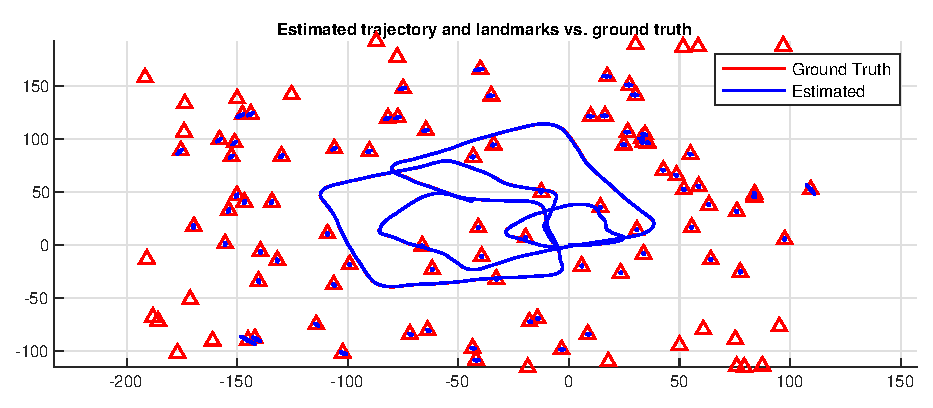
\includegraphics[width=0.7\linewidth]{figures/ga_3/sim_trajectory.eps}
    \caption{Estimated and ground truth pose trajectory and landmarks for simulated vehicle data}
    \label{fig:ga_3_sim_trajectory}
\end{figure}

\begin{figure}[!htb]
    \centering
    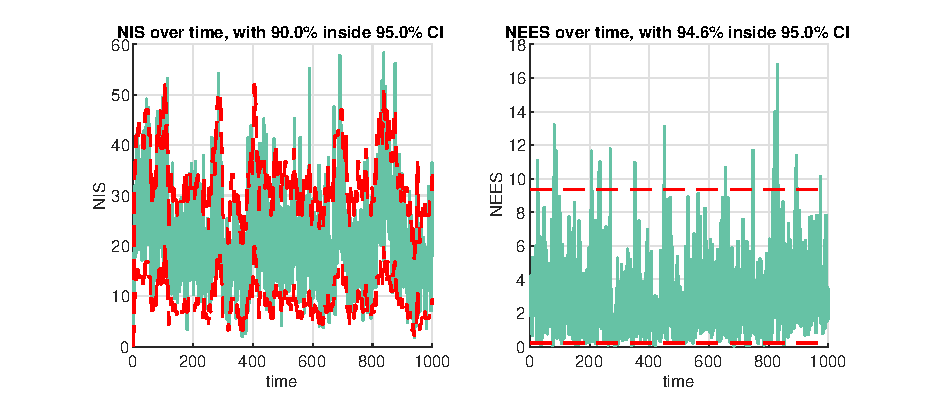
\includegraphics[width=0.9\linewidth]{figures/ga_3/sim_NIS.eps}
    \caption{Consistency for simulated vehicle data set with confidence intervals over time}
    \label{fig:ga_3_sim_NIS}
\end{figure}

Initially, the noise covariance matrices were set higher than necessary, to get a conservative result, and decreased until sufficient results were produced. At the same time, the compatibility alphas in the JCBB algorithm were reduced, as we could assume most of the measurements were from real landmarks.

% denseness, why?

%Discuss patterns in P - covariance. Discuss the two dots - why are these so high? They are not new states, but yet highly uncertain. It might just be the landmarks that are far away and that we have very few measurements off - might be the two landmarks with largest ellipses in trajectory plot? 
% Discuss using information matrix instead for speed? 

In \cref{fig:ga_3_sim_P} the covariance matrix and the inverse covariance matrix i.e. the information matrix at the last time step is presented. One should firstly note the denseness of the covariance matrix. This is a result of the fact that for the SLAM problem, all the states are highly correlated. We are trying to estimate the pose of the vehicle and the position of the landmarks relative to it simultaneously, which means that when we get additional information about the pose or a landmark from a measurement, we indirectly get information about all the other states as well. This means the covariance matrix will be very dense. Furthermore, we observe some additional structure in the covariance matrix, from the fact that landmarks that are close to each other will be more correlated than landmarks at different ends of the map. Finally, we also observe two outliers in the bottom right part of the diagonal. This might correspond to some of the landmarks in \cref{fig:ga_3_real_trajectory} with the largest covariance ellipses. These landmarks are far away from the trajectory of the vehicle and have therefore not been measured many times during the simulation. It then follows that they will be more uncertain than the rest and we get a few spikes in the covariance matrix.

Now consider the inverse of the covariance matrix i.e. the information matrix. When the covariance matrix is dense, the inverse matrix will naturally be sparse. As seen in \cref{fig:ga_3_sim_P} it is even approximately diagonal. This is a useful fact that could be used to reformulate the EKF equations in terms of the information matrix. This would be an interesting extension of the algorithm that might reduce computation time drastically. This reformulation is known in the literature as SEIF SLAM. 

\begin{figure}[!htb]
    \centering
    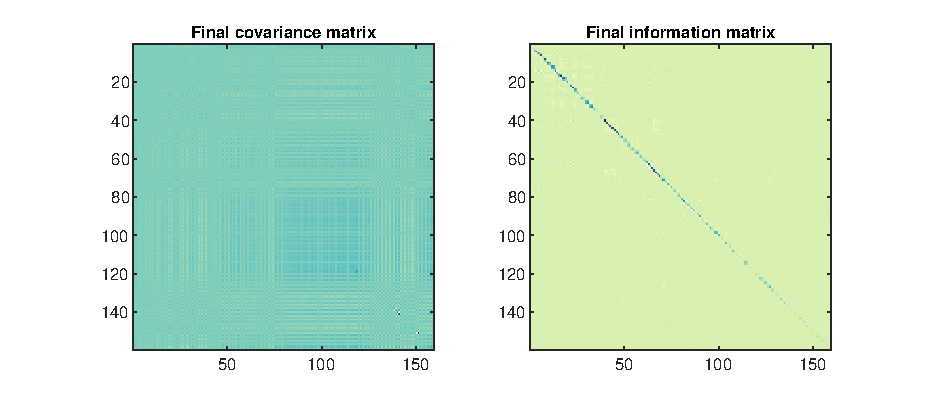
\includegraphics[width=0.8\linewidth]{figures/ga_3/sim_P.eps}
    \caption{Covariance matrix and information matrix for final timestep}
    \label{fig:ga_3_sim_P}
\end{figure}

% JCBB discussion

\subsection{EKF-SLAM on Victoria Park data set}

The EKF-SLAM code was then tested and tuned to the Victoria Park data set. The range-bearing measurement noise covariance was tuned with the same diagonal matrix, now with $\sigma_r = \SI{5e-2}{\meter}$ and $\sigma_\theta = \SI{5e-3}{rad}$. The odometer measurement noise covariance matrix was now tuned to be
\begin{equation}
    Q = \begin{bmatrix}
        0.25 & 0 & 0 \\
        0 & 0.25 & 0.0225 \\
        0 & 0.0225 & 0.0025 \\
    \end{bmatrix}.
\end{equation}
Notice how for this data set a high correlation between the measured sideways displacement $v$ and the measured heading $\varphi$. The JCBB individual and joint compatability significance levels were now tuned to be $\alpha_{ic} = \SI{1e-3}{}$ and $\alpha_{jc} = \SI{1e-3}{}$.

The system was largely tuned by the same process as for the simulated data, but there are several differences worth mentioning. Firstly, the pose ground truth is naturally no longer available, only GPS position measurements. This was plotted in relation to the estimated pose trajectory and landmarks, as seen in \cref{fig:ga_3_real_trajectory}. But there is no easy way to properly compare the estimate to the GPS measurement, as the EKF-SLAM algorithm only produces a local estimate in relation to how it was initialized. In \cref{fig:ga_3_real_trajectory} the GPS measurements were therefore rotated until the two different frames looked somewhat aligned.

\begin{figure}[!htb]
    \centering
    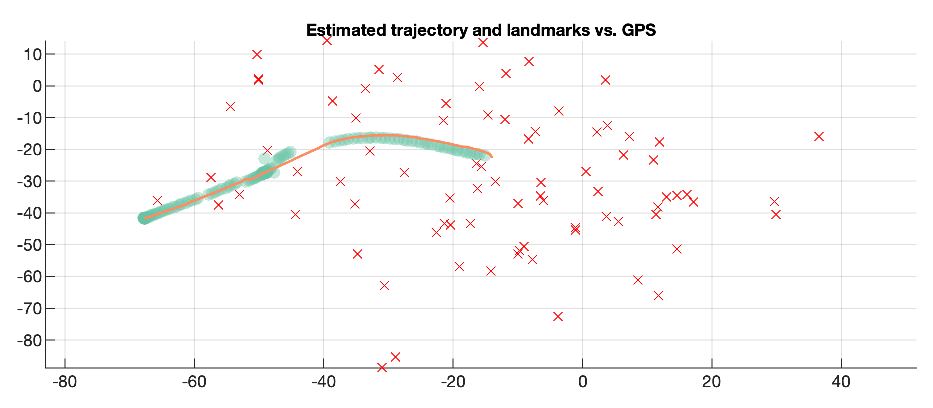
\includegraphics[width=0.7\linewidth]{figures/ga_3/real_trajectory.eps}
    \caption{Estimated pose trajectory, landmarks and GNSS measurements for Victoria Park data set}
    \label{fig:ga_3_real_trajectory}
\end{figure}

Since we no longer have the pose ground truth, the pose NEES is no longer available which also limits the available tools when tuning. But the NIS, again with a variable degree of freedom confidence interval, was actively used and is presented for the final tuning parameters in \cref{fig:ga_3_real_NIS}. It was calculated that 67\% of the NIS was inside the confidence intervals.  

\begin{figure}[!htb]
    \centering
    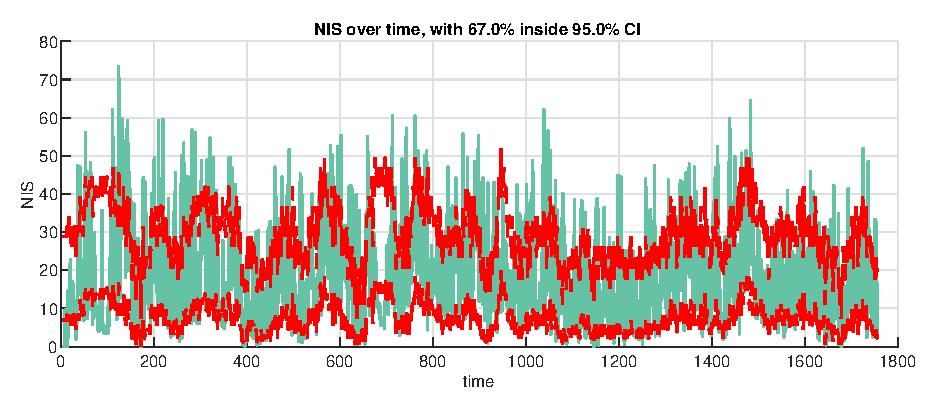
\includegraphics[width=0.8\linewidth]{figures/ga_3/real_NIS.eps}
    \caption{NIS for Victoria Park data set with confidence intervals over time}
    \label{fig:ga_3_real_NIS}
\end{figure}

One should also note the much higher compatibility alphas compared to the simulated data set. It was quickly observed while testing the system that the spread in range-bearing measurements of the landmarks was larger compared to the simulated case. It was concluded that the JCBB gating that was previously used was too low for this data set, and therefore increased. Another factor that influenced this tuning choice is the fact that each measurement that is not a part of the optimal choice with the most association matches from the JCBB algorithm are treated as new landmark states and added to the state vector. By increasing the individual and joint compatibility gate sizes we give JCBB more leeway, thereby reducing the number of new states added as the EKF-SLAM algorithm runs. Since, as previously discussed, the covariance matrix tends to be dense and very large, with a dimension in the hundreds, it is desirable to reduce the number of new states the algorithm adds to reduce computation time. It should be noted that JCBB will naturally use more time when the alphas are increased, as more association hypotheses must be considered. So how effective this strategy is in saving computation time is questionable, but this will slow down the growing state size which slows the algorithm down more and more over time, which was the primary concern here. 

% discuss EKF-SLAM assumptions.
% Discuss performance of EKF-SLAM. Why it sucks ass - fucked consistency and time scales with n^2 as we find more and more landmarks. Memory, quadratic scaling -> scales badly. Improvements, alternatives? Could decompose map into smaller independent maps? Robo-centric formulation? See book stuff. Different algorithms e.g. particle filter or graph-based approaches. 

When considering the performance of EKF-SLAM in these tests, one could argue that the performance is satisfactory, but several limitations are evident in the results. The first limitation, which applies to SLAM in general, is the fact that the estimated pose and landmark positions are only local estimates. While it is most important for the robot or vehicle to know its location relative to the environment, one can imagine several applications where global estimates are needed and this algorithm not being sufficient. One could remedy this by adding additional sensors to the system like a magnetometer, or simply making sure to initialize the system in the global frame. 

Another limitation is poor consistency, as a result of the fact that we are using an EKF. For the simulated data set the NEES did not evolve to be too large over time, but never the less it is a valid concern that the EKF will be too confident over time\cite{ekfslam}. One improvement to this is to formulate the EKF equations in a robocentric view. Alternatively, particle filter approaches or nonlinear observer theory can be used instead. 

Perhaps the more important limitation of EKF-SLAM is the memory and processing power requirements for the algorithm in large scale applications. Observe that the number of calculations and needed memory will scale quadratically for this algorithm. With the relatively small scale test using the Victoria Park data set, the script used about 10 minutes to finish $N=15000$ time steps, which corresponds to about 6,6 minutes of data, on a 2,7 GHz Intel Core i5. So for even this small scale example with only a few hundred landmarks the system was not able to operate in real-time. This demonstrates how infeasible it is to scale this algorithm to a more complex environment over a larger time horizon. For many applications, one can imagine that the number of landmarks could be several magnitudes larger than for this data set, and making it run online would not be feasible. This is not only because of the processing speed requirements but the memory requirements as well, when you have a dense covariance matrix consisting of millions of elements.

There are many possible improvements or alternatives that address these concerns. One idea is to simply separate the map into several independent parts to reduce the number of landmarks we are considering at the same time. This might allow us to better scale to a larger map. Reformulating the EKF-SLAM problem using the information matrix, as previously discussed, is also an alternative that could be explored. Graph-based methods are also based on the sparsity of the information matrix and could be used as an alternative to the EKF-SLAM. 

